La tabla comparativa proporciona información sobre los modelos planteados anteriormente, presentando de forma resumida sus Ventajas, Desventajas y Aplicaciones comunes de los modelos. Permitiendo tener una visión general de las características y consideraciones clave de cada modelo.

\begin{figure}[H]
    \begin{minipage}[t]{0.9\textwidth}
        \caption{Tabla comparativa modelos de predicción}
        \label{tabla_comparativa}        
    \end{minipage}

    \vspace{10pt}

    \begin{minipage}[b]{0.99\textwidth}
        \centering
        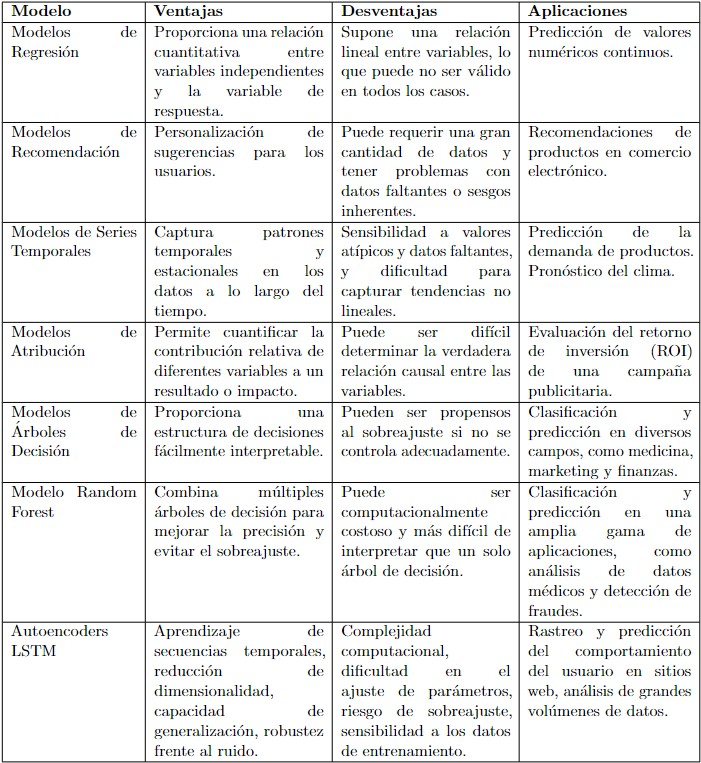
\includegraphics[width=\textwidth]{img/tabla comparativa modelos.jpg}        
    \end{minipage}

    \begin{minipage}[t]{0.9\textwidth}
        Fuente: Elaboración propia.
    \end{minipage}
\end{figure}

% \begin{table}[ht]
% \captionsetup{font=small} % Ajusta el tamaño de fuente de la leyenda de la tabla
% \small % Ajusta el tamaño de fuente de la tabla
% \begin{tabular}{|p{0.2\linewidth}|p{0.27\linewidth}|p{0.27\linewidth}|p{0.26\linewidth}|}
% \hline
% \textbf{Modelo} & \textbf{Ventajas} & \textbf{Desventajas} & \textbf{Aplicaciones} \\
% \hline
% Modelos de Regresión & 
% Proporciona una relación cuantitativa entre variables independientes y la variable de respuesta. & 
% Supone una relación lineal entre variables, lo que puede no ser válido en todos los casos. & 
% Predicción de valores numéricos continuos. \\
% \hline
% Modelos de Recomendación & 
% Personalización de sugerencias para los usuarios. & 
% Puede requerir una gran cantidad de datos y tener problemas con datos faltantes o sesgos inherentes. & 
% Recomendaciones de productos en comercio electrónico. \\
% \hline
% Modelos de Series Temporales & 
% Captura patrones temporales y estacionales en los datos a lo largo del tiempo. & 
% Sensibilidad a valores atípicos y datos faltantes, y dificultad para capturar tendencias no lineales. & 
% Predicción de la demanda de productos. Pronóstico del clima. \\
% \hline
% Modelos de Atribución & 
% Permite cuantificar la contribución relativa de diferentes variables a un resultado o impacto. & 
% Puede ser difícil determinar la verdadera relación causal entre las variables. & 
% Evaluación del retorno de inversión (ROI) de una campaña publicitaria. \\
% \hline
% Modelos de Árboles de Decisión & 
% Proporciona una estructura de decisiones fácilmente interpretable. & 
% Pueden ser propensos al sobreajuste si no se controla adecuadamente. & 
% Clasificación y predicción en diversos campos, como medicina, marketing y finanzas. \\
% \hline
% Modelo Random Forest & 
% Combina múltiples árboles de decisión para mejorar la precisión y evitar el sobreajuste. & 
% Puede ser computacionalmente costoso y más difícil de interpretar que un solo árbol de decisión. & 
% Clasificación y predicción en una amplia gama de aplicaciones, como análisis de datos médicos y detección de fraudes. \\
% \hline
% \end{tabular}
% \end{table}
